In the original publication of the DBSCAN algorithm \cite{dbscan} a simple way for approximating the minPts and eps parameters was proposed.

The described heuristic defines a function \texttt{k-dist} which calculates the distance d of each point to its k-nearest neighbour.
The d-neighbourhood of each point then contains k+1 points in most cases. Theoretically it could happen that two points share the same distance d to a point. Then the d-neighbourhood could contain more than k+1 points though this case is most unlikely.

Sorting the resulting distances in decending order and plotting them against the points results in the so called sorted k-dist graph. This graph gives some insights about the datasets density distribution. Choosing any point in this graph, setting minPts to k and eps to the k-dist value of the point will result in DBSCAN classifing every point with the same or smaller k-dist value as core point. These points will therefore be assigned to a cluster. Points with a larger k-dist value could be, but do not have to be, classified as noise. 

In the sorted k-dist graph a threshold point can be searched describing the maximal distance of the thinnest cluster. The DBSCAN paper \cite{dbscan} proposes a visual approach on finding such threshold points by looking for a kind of bend or "valley" in the graph. 
In figure \ref{fig:sorteddistgraphiriseucl} an example is shown for such a bend found in the 4-dist graph of the iris dataset using the euclidean distance.

\begin{figure}
    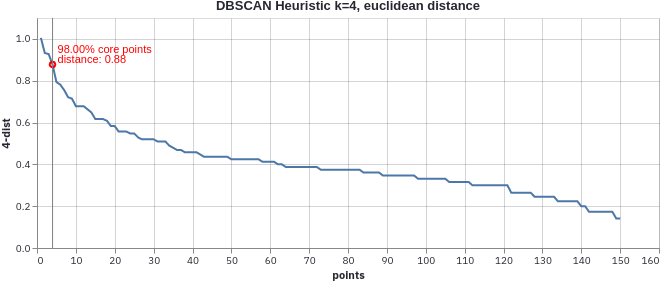
\includegraphics[width=0.92\textwidth]{../plots/dbscan/iris_4dist_euclidean}
    \caption{sorted 4-dist graph for iris dataset and euclidean distance}
    \label{fig:sorteddistgraphiriseucl}
\end{figure}

While this method provides good results for some datasets, sometimes the estimated parameters do not produce a meaningful clustering or a bend may not be visible in the sorted k-dist graph. In some cases the distance chosen may result in one large cluster. The eps must then be reduced until DBSCAN can find multiple clusters, most likely resulting in more noise.

An interactive display of this heuristic with adjustable parameters for all datasets was also created using streamlit and altair and is hosted on streamlit sharing 
\footnote{\scriptsize\url{https://share.streamlit.io/elpelt/datascience1_group42/main/code/heuristic_web.py}}
The plot in figure \ref{fig:sorteddistgraphiriseucl} was created using this interface.
